\documentclass[tikz,border=10pt]{standalone}
\usepackage{pgfplots}
% Necessário para compatibilidade com os padrões mais recentes do pgfplots
\pgfplotsset{compat=1.18} 

\begin{document}
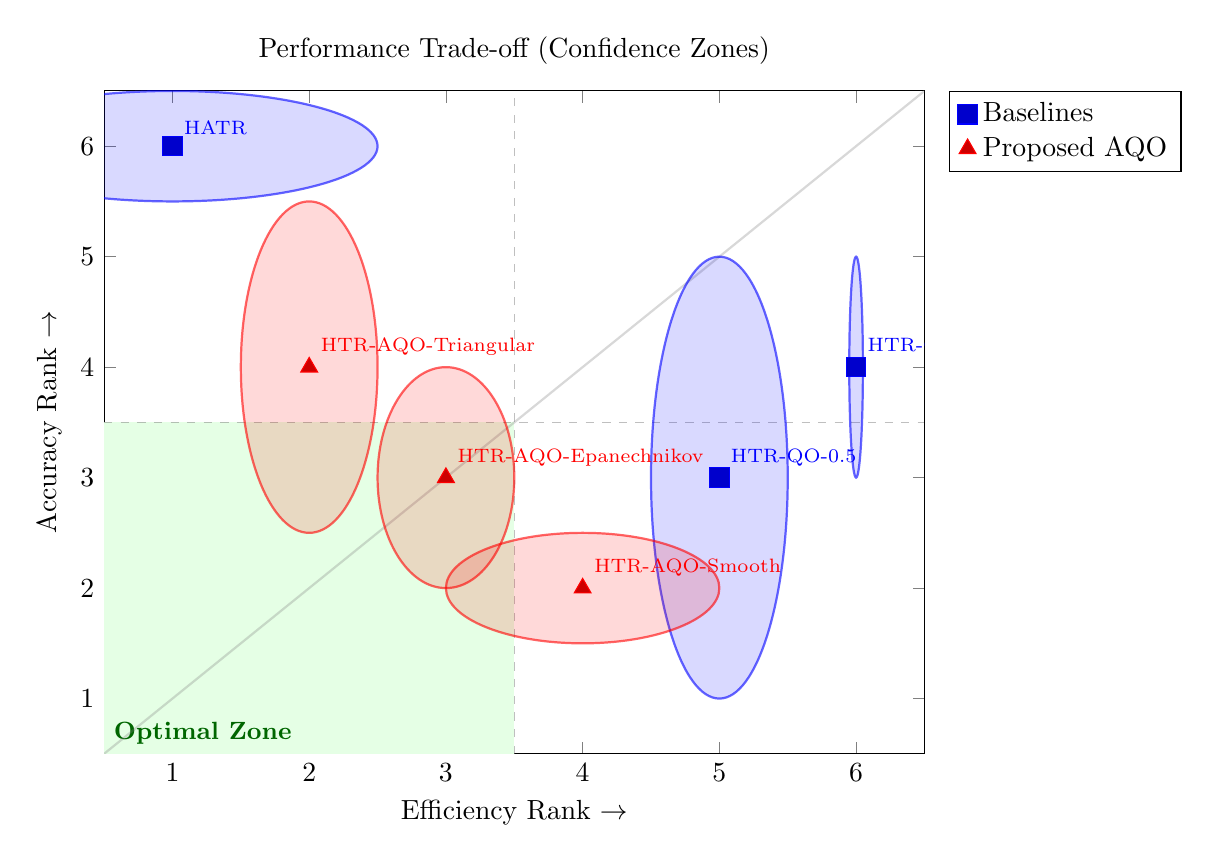
\begin{tikzpicture}
  \begin{axis}[
    width=12cm, height=10cm,
    xlabel={Efficiency Rank $\rightarrow$},
    ylabel={Accuracy Rank $\rightarrow$},
    title={Performance Trade-off (Confidence Zones)},
    legend pos=outer north east,
    legend cell align={left},
    xmin=0.5, xmax=6.5,
    ymin=0.5, ymax=6.5,
    axis background/.style={fill=white},
    axis on top=false,
  ]

  % Optimal Zone Background
  \fill[green!10] (0.5, 0.5) rectangle (3.50, 3.50);
  \node[text=black!60!green, above right, font=\small\bfseries] at (0.5, 0.5) {Optimal Zone};\n\n  % Grid Lines and Equilibrium
  \draw[gray, dashed, opacity=0.5] (0.5, 3.50) -- (6.5, 3.50);
  \draw[gray, dashed, opacity=0.5] (3.50, 0.5) -- (3.50, 6.5);
  \addplot[gray, thick, opacity=0.3, mark=none, forget plot] coordinates {(0.5,0.5) (6.5,6.5)};

  % Confidence Ellipses (IQR)
  \filldraw[fill=blue, draw=blue, fill opacity=0.15, draw opacity=0.6, thick] (1.00, 6.00) ellipse [x radius=1.50, y radius=0.50];
  \filldraw[fill=blue, draw=blue, fill opacity=0.15, draw opacity=0.6, thick] (6.00, 4.00) ellipse [x radius=0.05, y radius=1.00];
  \filldraw[fill=blue, draw=blue, fill opacity=0.15, draw opacity=0.6, thick] (5.00, 3.00) ellipse [x radius=0.50, y radius=2.00];
  \filldraw[fill=red, draw=red, fill opacity=0.15, draw opacity=0.6, thick] (2.00, 4.00) ellipse [x radius=0.50, y radius=1.50];
  \filldraw[fill=red, draw=red, fill opacity=0.15, draw opacity=0.6, thick] (3.00, 3.00) ellipse [x radius=0.50, y radius=1.00];
  \filldraw[fill=red, draw=red, fill opacity=0.15, draw opacity=0.6, thick] (4.00, 2.00) ellipse [x radius=1.00, y radius=0.50];

  % Markers and Legends
  \addplot+[blue, only marks, mark=square*, mark size=3.5] coordinates {
    (1.00, 6.00)
    (6.00, 4.00)
    (5.00, 3.00)
  };
  \addlegendentry{Baselines}

  \node[above right, inner sep=4pt, text=blue, font=\scriptsize] at (1.00, 6.00) {HATR};
  \node[above right, inner sep=4pt, text=blue, font=\scriptsize] at (6.00, 4.00) {HTR-QO-0.25};
  \node[above right, inner sep=4pt, text=blue, font=\scriptsize] at (5.00, 3.00) {HTR-QO-0.5};
  \addplot+[red, only marks, mark=triangle*, mark size=3.5] coordinates {
    (2.00, 4.00)
    (3.00, 3.00)
    (4.00, 2.00)
  };
  \addlegendentry{Proposed AQO}

  \node[above right, inner sep=4pt, text=red, font=\scriptsize] at (2.00, 4.00) {HTR-AQO-Triangular};
  \node[above right, inner sep=4pt, text=red, font=\scriptsize] at (3.00, 3.00) {HTR-AQO-Epanechnikov};
  \node[above right, inner sep=4pt, text=red, font=\scriptsize] at (4.00, 2.00) {HTR-AQO-Smooth};
  \end{axis}
\end{tikzpicture}

\end{document}
